
\documentclass[hyperref={pdfpagelabels=false},ngerman]{beamer}

% stop font warning
\let\Tiny=\tiny
\providecommand\thispdfpagelabel[1]{}

\usepackage[english]{babel}
\usepackage{lmodern}
\usepackage[T1]{fontenc}
\usepackage[utf8]{inputenc}
\usepackage{graphicx,import}
\usepackage{feynmp}
\DeclareGraphicsRule{*}{mps}{*}{} 
\DeclareGraphicsExtensions{.pdf}
\usepackage{amsmath,amssymb,amstext,amsfonts} % mathrsfs
\usepackage{array,booktabs,tabularx}
\usepackage{tikz,tikz-uml,pgf-pie}
\usetikzlibrary{shapes,calc,arrows,positioning}
\tikzstyle{block} = [rectangle, draw, text width=7em, text centered, minimum height=2em]
\tikzstyle{arrow} = [draw, -latex, thick]
\tikzstyle{arrow2} = [draw, latex-latex, thick]
\tikzstyle{quark}  = [rectangle, draw, fill=yellow, minimum width=2em, text centered, minimum height=2em]
\tikzstyle{lepton} = [rectangle, draw, fill=red!50, minimum width=2em, text centered, minimum height=2em]
\tikzstyle{gauge}  = [circle   , draw, fill=green , minimum size=2em, inner sep=0pt, text centered]
\tikzstyle{scalar} = [diamond  , draw, fill=blue!40, minimum width=2.3em, text centered, minimum height=2.3em, inner sep=0pt]
\tikzstyle{goldstone} = [diamond, draw, dashed, fill=blue!30, minimum width=2.3em, text centered, minimum height=2.3em, inner sep=0pt]
\tikzstyle{squark}   = [diamond, draw, fill=yellow, minimum width=2.3em, text centered, minimum height=2.3em, inner sep=0pt]
\tikzstyle{slepton}  = [diamond, draw, fill=red!50, minimum width=2.3em, text centered, minimum height=2.3em, inner sep=0pt]
\tikzstyle{gaugino}  = [rectangle, draw, fill=green , minimum size=2em, inner sep=0pt, text centered]
\tikzstyle{higgsino} = [rectangle, draw, fill=blue!40  , minimum width=2em, text centered, minimum height=2em]
\tikzstyle{inert}    = [diamond  , draw, fill=teal!80, minimum width=2.3em, text centered, minimum height=2.3em, inner sep=0pt]
\tikzstyle{inertino} = [rectangle, draw, fill=teal!80, minimum width=2em, text centered, minimum height=2em]
\tikzstyle{phantom}  = [rectangle, minimum width=2em, text centered, minimum height=2em]
\usepackage{slashed}
\usepackage{fixltx2e} % textsubscript
\usepackage{multirow}
\usepackage{tcolorbox}
\usepackage{pifont}
\usepackage{xspace}
\usepackage{hyperref}
\hypersetup{colorlinks,linkcolor=,urlcolor=blue}
\usepackage{listings}
\lstset{breaklines=true,
  breakatwhitespace=true,
%  numbers=left,
  numberstyle=\tiny,
  stepnumber=1,
  basicstyle=\ttfamily\footnotesize,
  commentstyle=\ttfamily\color{gray},
  postbreak={\mbox{{$\hookrightarrow$}}\space\space},
  breakindent=10pt,
  breakautoindent=false,
  showspaces=false,
  showstringspaces=false,
  frame=single}

\definecolor{darkgreen}{RGB}{0,176,0}

\newcommand{\cmark}{\ding{51}}%
\newcommand{\xmark}{\ding{55}}%
\newcommand{\fmfvcenter}[1]{\;\vcenter{\hbox{\fmfreuse{#1}}}\;}
\newcommand{\eh}[1]{\,\mathsf{#1}}
\newcommand{\ok}{\textcolor{darkgreen}{\cmark}}
\newcommand{\notok}{\textcolor{red}{\xmark}}
\newcommand{\maybe}{\textcolor{gray}{\cmark}}
\newcommand{\Lagr}{\mathcal{L}}
\newcommand{\mathi}{\mathsf{i}}
\newcommand{\mycite}[1]{\textcolor{darkgray}{\tiny [#1]}}
\newcommand{\bigcite}[1]{\textcolor{darkgray}{[#1]}}
\newcommand{\dimrep}[1]{\mathbf{#1}}
\newcommand{\dimrepadj}[1]{\mathbf{\overline{#1}}}
\newcommand{\ESSM}{E\textsubscript{6}SSM}
\newcommand{\CESSM}{CE\textsubscript{6}SSM}
\DeclareMathOperator{\tildeRe}{\widetilde Re}
\DeclareMathOperator{\sign}{sign}
\DeclareMathOperator{\re}{Re}
\DeclareMathOperator{\im}{Im}
\renewcommand{\emph}{\textbf}
\newcommand{\dd}{\mathsf{d}}
\newcommand{\myurl}[1]{\href{#1}{#1}}
\newcommand{\Superpot}{\mathcal{W}}
\newcommand{\SuperField}[1]{#1}
\newcommand{\ConjSuperField}[1]{\bar{#1}}
\newcommand{\UY}{\ensuremath{U(1)_{Y}}}
\newcommand{\UN}{\ensuremath{U(1)_{N}}}
\newcommand{\Uem}{\ensuremath{U(1)_\text{em}}}
\newcommand{\SUL}{\ensuremath{SU(2)_\text{L}}}
\newcommand{\SUc}{\ensuremath{SU(3)_\text{c}}}
\newcommand{\SOten}{\ensuremath{{SO(10)}}}
\newcommand{\comma}{,}
\newcommand{\DRbar}{\ensuremath{\overline{\text{DR}}}}
\newcommand{\MSbar}{\ensuremath{\overline{\text{MS}}}}
\newcommand{\SM}{\ensuremath{\text{SM}}}
\newcommand{\MSSM}{\ensuremath{\text{MSSM}}}
\newcommand{\pole}{\ensuremath{\text{pole}}}
\newcommand{\tree}{\ensuremath{\text{tree}}}
\newcommand{\Zv}{\ensuremath{\backslash\mkern-11.0mu{Z_3}}}
\newcommand{\downrightknickarrow}{\mathrel{\scalebox{1.3}{\rotatebox[origin=c]{180}{$\Lsh$}}}}
\newcommand{\threelinebrace}{$\left. \begin{array}{c} \\ \\ \\ \end{array} \right\rbrace$}
\newcommand{\fivelinebrace}{$\left. \begin{array}{c} \\ \\ \\ \\ \\ \end{array} \right\rbrace$}
\newcommand{\twolinebrace}{$\left. \begin{array}{c} \\ \\ \end{array} \right\rbrace$}
\newcommand{\elevenlinebrace}{$\left. \begin{array}{c} \\ \\ \\ \\ \\ \\ \\ \\ \\ \\ \\ \end{array} \right\rbrace$}

% set look of slides
\usetheme{Madrid}
\useoutertheme{default}
\useinnertheme{circles}
\usecolortheme{default}
\beamertemplatenavigationsymbolsempty % keine Navigationselemente
\setbeamersize{text margin left = 1cm, text margin right = 1cm}

% define footer
\makeatletter
\setbeamertemplate{footline}
{
  \hfill\hbox{\insertframenumber{} / \inserttotalframenumber\hspace*{4pt}}%
  \vskip3pt%
}
\makeatother
\usecolortheme{tud}

\title{Higgs mass calculations in supersymmetry at the 2-loop level
  for high and low SUSY scales}

\author[Alexander Voigt]{Peter Athron, Thomas Kwasnitza, Jae-hyeon Park, Tom Steudtner, Dominik Stöckinger, \underline{Alexander Voigt}}

\date{23.--25.01.2017}

\institute[Aachen]{KUTS-6, Aachen 2017}
\subject{FlexibleSUSY,MSSM,Higgs,FlexibleEFTHiggs}
\keywords{FlexibleSUSY,MSSM,Higgs,FlexibleEFTHiggs}

%%%%%%%%%%%%%%%%%%%%%%%%%%%%%%%%%%%%%%%%%%%%%%%%%%%%%%%%%%%%%%%%%%%%%%%%%%%%%

\begin{document}

%%%%%%%%%%%%%%%%%%%%%%%%%%%%%%%%%%%%%%%%
\begin{frame}[plain]
  \tikz [remember picture,overlay]
  \node at
    ([yshift=1.3cm,xshift=4cm]current page.south)
    {
\includegraphics[height=2cm]{images/RWTH_Logo}};
  \titlepage  
  % \vspace*{1em}
  % \centering In collaboration with Peter Athron, Jae-hyeon Park and Dominik Stöckinger [\href{https://arxiv.org/abs/1406.2319}{arxiv:1406:2319}] 
\end{frame}

%%%%%%%%%%%%%%%%%%%%%%%%%%%%%%%%%%%%%%%%
\begin{frame}{Contents}
  \tableofcontents
\end{frame}

\section{What is FlexibleSUSY?}

\begin{frame}{Contents}
  \tableofcontents[currentsection]  
\end{frame}

\begin{frame}{FlexibleSUSY = spectrum generator generator}
  \begin{center}
    FlexibleSUSY~~~~~\\
    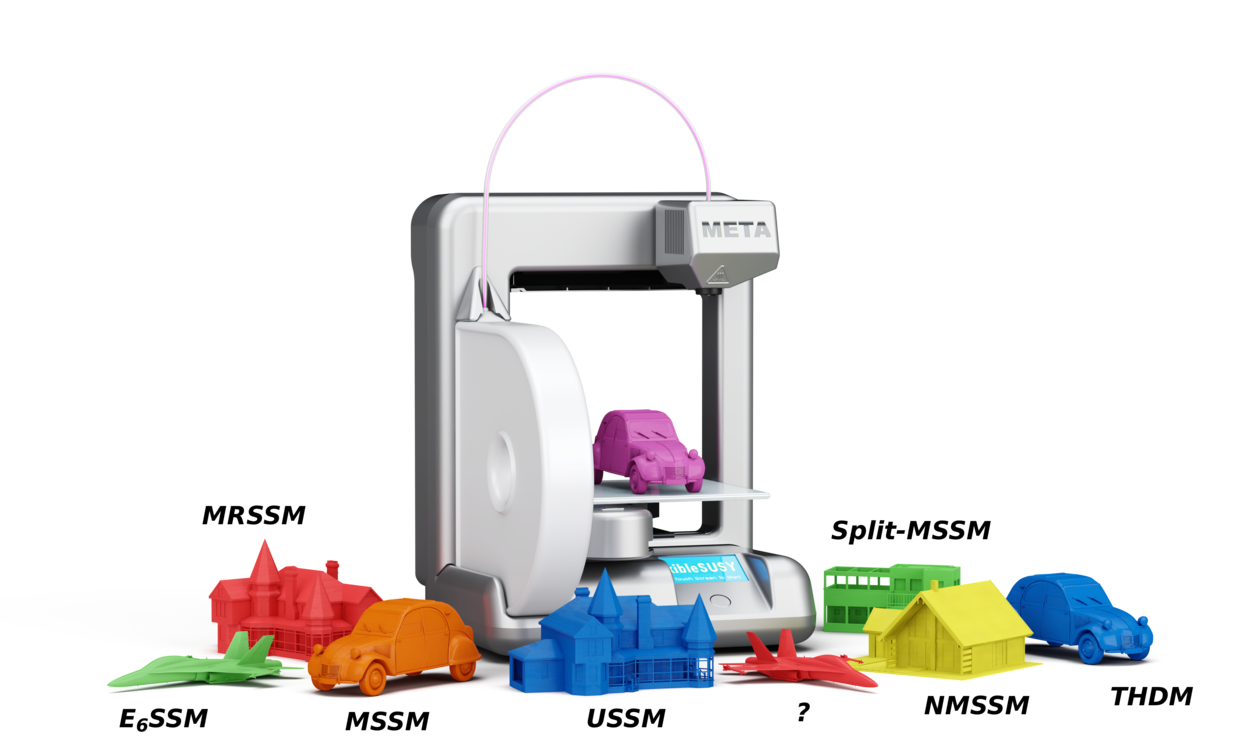
\includegraphics[width=\textwidth]{images/FS.png}
  \end{center}
\end{frame}

%%%%%%%%%%%%%%%%%%%%%%%%%%%%%%%%%%%%%%%%

\section{Approaches to predict $M_h$}

\begin{frame}{Contents}
  \tableofcontents[currentsection]  
\end{frame}

\subsection{Full model approach}

\begin{frame}{Full model approach}
  \begin{center}
    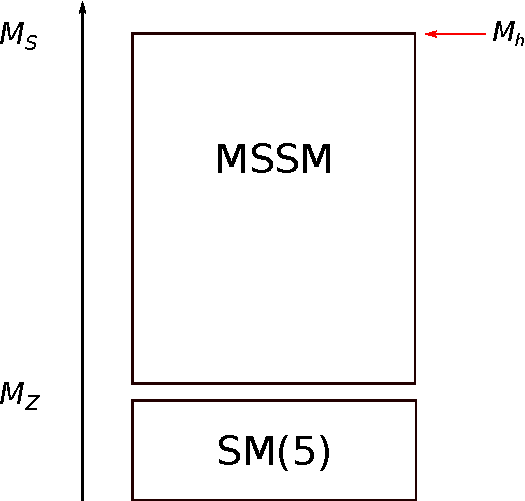
\includegraphics[width=0.45\textwidth]{images/mssm-sm-tower-diagrammatic}\\[1em]
  \end{center}
  \emph{Idea:} Calculate $M_h$ in the MSSM at the scale $Q = M_S$ as a function of the \DRbar\ parameters:\\[1em]
  \centering $g_i$, $y^f_{ij}$, $v_i$, $\mu$, $B\mu$, $m^2_{H_i}$,
  $m_{\tilde{f},ij}^2$, $M_i$, $T^f_{ij}$
\end{frame}

\begin{frame}{Full model approach}
  \begin{align*}
    (M_h^\text{MSSM})^2 &= \text{smallest eigenvalue of} \\
    &\phantom{={}} \left[(m_h^\text{MSSM})^2 - \Sigma^\text{MSSM}_h((M_h^\text{MSSM})^2,M_S)
      + \frac{t_h^\text{MSSM}}{v}\right]_{ij}
  \end{align*}
  \emph{Advantage:} includes all 1L terms $O(p^2/M_S^2)$\\
  \emph{Disadvantage:} suffers from large logarithms $\propto\log(M_t/M_S)$ if $M_S\gg M_t$\\
\end{frame}

%%%%%%%%%%%%%%%%%%%%%%%%%%%%%%%%%%%%%%%%

\begin{frame}{EFT approach}
  \begin{center}
    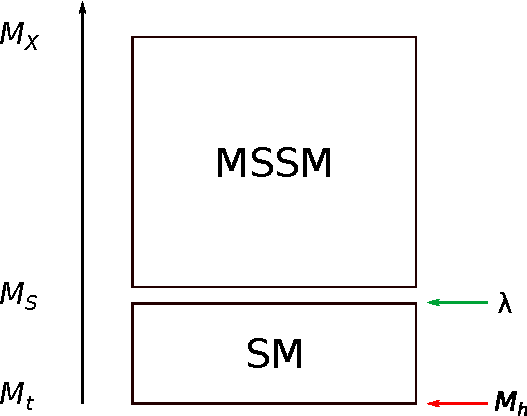
\includegraphics[width=0.45\textwidth]{images/mssm-sm-tower-eft}\\[1em]
  \end{center}
  \emph{Idea:} Calculate $M_h$ in the SM at the scale $Q = M_t$ as a function of the \MSbar\ parameters:\\[1em]
  \centering $g_i$, $y^f_{ij}$, $v$, $\mu^2$, $\lambda$
\end{frame}

%%%%%%%%%%%%%%%%%%%%%%%%%%%%%%%%%%%%%%%%

\subsection{EFT approach with $\Gamma$ matching}

\begin{frame}{EFT approach with $\Gamma$ matching}
  Determine $\lambda(M_S)$ from mathching all
  $\Gamma_{\phi_1,\ldots,\phi_n}^{(k)}(p^2 = 0, Q = M_S)$: $\Rightarrow$
  \begin{align*}
    \lambda (M_S) &= \frac{1}{4}\left[g_Y^{2} + g_2^2\right] \cos^22\beta
    + \Delta \lambda
  \end{align*}
  RG running to $Q=M_t$ $\Rightarrow$
  \begin{align*}
    (M_h^\SM)^2 &= \lambda v^2 - \Sigma^\SM_h((M_h^\SM)^2) + \frac{t_h^\SM}{v}
  \end{align*}
  \emph{Advantage:} resums large logarithms $\propto\log(M_t/M_S)$\\
  \emph{Disadvantage:} difficult to automatize; neglects terms
  $O(p^2/M_S^2)$ from SUSY particles if performed at 1L-level only
\end{frame}

%%%%%%%%%%%%%%%%%%%%%%%%%%%%%%%%%%%%%%%%

\subsection{EFT approach with $M_h$ matching (FlexibleEFTHiggs)}

\begin{frame}{EFT approach with $M_h$ matching (FlexibleEFTHiggs)}
  \begin{align*}
    M_h^{\SM} &\overset{!}{=} M_h^\text{MSSM} \quad \text{at} \quad Q = M_S, 1L/2L
  \end{align*}
  $\Rightarrow$
  \begin{align*}
    \lambda \leftarrow \frac{1}{v^2} \left[
      (m_h^\SM)^2 + (M_h^\text{MSSM})^2 - (M_h^\SM)^2
    \right]
  \end{align*}
  3-loop RG running to $Q = M_t$:
  \begin{align*}
    M_h^2 &= \lambda v^2 - \Sigma^{\SM}_h(M_h^2) + \frac{t_h^\SM}{v}
    \qquad \text{(1L/2L)}
  \end{align*}
\end{frame}

\begin{frame}{EFT approach with $M_h$ matching (FlexibleEFTHiggs)}
  Matching condition for $y_t$:
  \begin{align*}
    M_t^{\SM} &\overset{!}{=} M_t^\text{MSSM} \quad \text{at} \quad Q = M_S, 2L
  \end{align*}
  $\Rightarrow$
  \begin{align*}
    y_t^\MSSM \leftarrow \frac{\sqrt{2}}{v_u} \left[
      m_t^\MSSM - M_t^\MSSM + M_t^\SM
    \right]
  \end{align*}
  Matching conditions for $g_i$:
  \begin{align*}
    &M_V^{\SM} \overset{!}{=} M_V^\text{MSSM} \quad \text{at} \quad Q = M_S, 1L \quad (V = W,Z)\\
    &\alpha_{\text{em}}^\MSSM(M_S) = \alpha_{\text{em}}^\SM(M_S) \ (1 + \Delta\alpha_{\text{em}})\\
    &\alpha_s^\MSSM(M_S) = \alpha_s^\SM(M_S)
  \end{align*}
\end{frame}

%%%%%%%%%%%%%%%%%%%%%%%%%%%%%%%%%%%%%%%%

\begin{frame}{Incorrect 2L logs in FlexibleEFTHiggs-1L}
  Matching condition:
  \begin{align*}
    \lambda &\leftarrow \frac{1}{v^2} \left[
      (m_h^\SM)^2 + (M_h^\text{MSSM})^2 - (M_h^\SM)^2
    \right]
  \end{align*}
  Expansion of momentum iteration up to 1L level:
  \begin{align*}
    \lambda &= \frac{1}{v^2} \Big[
      (m_h^\MSSM)^2
      + \Delta m_{h,\MSSM}^2
      - \Delta m_{h,\SM}^2
      + O(\hbar^2)
    \Big]
  \end{align*}
  with
  \begin{align*}
    \Delta m_{h,\MSSM}^2 &= -\Sigma^{1L}_{\MSSM} + t_{\MSSM}^{1L}/v_\MSSM \\
    \Delta m_{h,\SM}^2 &= -\Sigma^{1L}_{\SM} + t^{1L}_{\SM}/v_\SM
  \end{align*}
\end{frame}

\begin{frame}{Incorrect 2L logs in FlexibleEFTHiggs-1L}
  \emph{Problem:} $y_t^{\MSSM} = y_t^\SM/s_\beta [1 + O(\hbar)] $\\
  $\Rightarrow$
  \begin{align*}
    \Delta m_{h,\MSSM}^2 - \Delta m_{h,\SM}^2 &\propto
    \hbar \Bigg[ (y_t^\MSSM s_\beta)^4 \log\frac{m_t}{M_S} - (y_t^\SM)^4 \log\frac{m_t}{M_S}\Bigg] \\
    &= \hbar \Bigg[0\ + \propto \hbar y_t^4 \log\frac{m_t}{M_S} + O(\hbar^2) \Bigg] \\
    &= O(\hbar^2 y_t^4 \log\frac{m_t}{M_S})
  \end{align*}
  $\Rightarrow$\\
  incorrect 2L logs remain in FlexibleEFTHiggs-1L\\[1em]
  $\Rightarrow$\\
  FlexibleEFTHiggs-1L: incorrect 2L logs $O(\hbar^2 \log(M_t/M_S))$
  FlexibleEFTHiggs-2L: incorrect 3L logs $O(\hbar^3 \log^2(M_t/M_S))$
\end{frame}

%%%%%%%%%%%%%%%%%%%%%%%%%%%%%%%%%%%%%%%%

\begin{frame}{EFT approach with $M_h$ matching (FlexibleEFTHiggs)}
  \emph{Advantages:}
  \begin{itemize}
  \item easily automatizable
  \item FlexibleEFTHiggs-1L/2L correctly resums LL
  \item FlexibleEFTHiggs-1L: all non-log terms correct at 1L, \\
    including all terms $O(p^n/M_S^n, v^n/M_S^n)$
  \item FlexibleEFTHiggs-2L: non-log terms correct at 2L
    $O(\alpha_s(\alpha_t + \alpha_b) + (\alpha_t + \alpha_b)^2 + \alpha_\tau^2)$
  \end{itemize}
  \emph{Disadvantage:}
  \begin{itemize}
  \item FlexibleEFTHiggs-1L: incorrect 2L logs $O(\hbar^2 \log(M_t/M_S))$
  \item FlexibleEFTHiggs-2L: incorrect 3L logs $O(\hbar^3 \log^2(M_t/M_S))$
  \end{itemize}
\end{frame}

%%%%%%%%%%%%%%%%%%%%%%%%%%%%%%%%%%%%%%%%

\section{Numerical comparison of the approaches}

\begin{frame}{Contents}
  \tableofcontents[currentsection]  
\end{frame}

\begin{frame}{Numerical comparison}
  \begin{figure}
    \centering
    \includegraphics[width=\textwidth]{plots/FlexibleEFTHiggs/Mh_MS_TB-5_Xt-0}
  \end{figure}
  $\tan\beta = 5$, $X_{t,b,\tau} = 0$
\end{frame}

\begin{frame}{Numerical comparison}
  \begin{figure}
    \centering
    \includegraphics[width=\textwidth]{plots/FlexibleEFTHiggs/Mh_relative_MS_TB-5_Xt-0}
  \end{figure}
  $\tan\beta = 5$, $X_{t,b,\tau} = 0$
\end{frame}

\begin{frame}{Numerical comparison}
  \begin{figure}
    \centering
    \includegraphics[width=\textwidth]{plots/FlexibleEFTHiggs/Mh_Xt_TB-5_MS-2000}
  \end{figure}
  $\tan\beta = 5$, $M_S = 2 \eh{TeV}$, $X_{b,\tau} = 0$
\end{frame}

\begin{frame}{Numerical comparison}
  \begin{figure}
    \centering
    \includegraphics[width=\textwidth]{plots/FlexibleEFTHiggs/Mh_relative_Xt_TB-5_MS-2000}
  \end{figure}
  $\tan\beta = 5$, $M_S = 2 \eh{TeV}$, $X_{b,\tau} = 0$
\end{frame}

%%%%%%%%%%%%%%%%%%%%%%%%%%%%%%%%%%%%%%%%

\section{Uncertainty estimation}

\begin{frame}{Uncertainty estimation of FlexibleEFTHiggs}
  \begin{itemize}
  \item relation between $y_t^{\text{SM}}$ and $y_t^{\text{MSSM}}$ one loop order higher \\
    FlexibleEFTHiggs-1L: $\rightarrow$ $\Delta M_h^{(y_t\ \text{0L vs. 1L})}$\\
    FlexibleEFTHiggs-2L: $\rightarrow$ $\Delta M_h^{(y_t\ \text{1L vs. 2L})}$
  \item variation of $Q_\text{match}$ within $[M_S/2, 2 M_S]$ \\
    $\rightarrow$ $\Delta M_h^{(Q_\text{match})}$
  \item variation of $Q_\text{pole}$ within $[M_t/2, 2 M_t]$ \\
    $\rightarrow$ $\Delta M_h^{(Q_\pole)}$
  \end{itemize}
\end{frame}

\begin{frame}{Uncertainty estimation of FlexibleEFTHiggs}
  \begin{minipage}[t]{0.49\textwidth}
    \centering
    1-loop \\
    \includegraphics[width=\textwidth]{plots/FlexibleEFTHiggs/DMh_tower-1L_MS_TB-5_Xt-0}\\
    \includegraphics[width=\textwidth]{plots/FlexibleEFTHiggs/DMh_tower-1L_Xt_TB-5_MS-2000}
  \end{minipage}\hfill
  \begin{minipage}[t]{0.49\textwidth}
    \centering
    2-loop \\
    \includegraphics[width=\textwidth]{plots/FlexibleEFTHiggs/DMh_tower-2L_MS_TB-5_Xt-0}\\
    \includegraphics[width=\textwidth]{plots/FlexibleEFTHiggs/DMh_tower-2L_Xt_TB-5_MS-2000}
  \end{minipage}
\end{frame}

\begin{frame}{FlexibleEFTHiggs 2L combined uncertainty}
  \begin{figure}
    \centering
    \includegraphics[width=\textwidth]{plots/FlexibleEFTHiggs/Mh_uncertainties_relative_MS_TB-5_Xt-0}
  \end{figure}
  $\tan\beta = 5$, $X_{t,b,\tau} = 0$
\end{frame}

\begin{frame}{FlexibleEFTHiggs 2L combined uncertainty}
  \begin{figure}
    \centering
    \includegraphics[width=\textwidth]{plots/FlexibleEFTHiggs/Mh_uncertainties_relative_Xt_TB-5_MS-2000}
  \end{figure}
  $\tan\beta = 5$, $X_{t,b,\tau} = 0$
\end{frame}

%%%%%%%%%%%%%%%%%%%%%%%%%%%%%%%%%%%%%%%%

\section{Summary}

\begin{frame}{Summary}
  \begin{itemize}
  \item full model approach suffers from large logs
    $\propto\log(M_t/M_S)$ if $M_S \gg M_t$
  \item pure EFT approach resums N$^n$LL but neglects terms
    $O(p^2/M_S^2)$.  Also difficult to automatize.
  \item FlexibleEFTHiggs
    \begin{itemize}
    \item resums LL (but incorrect NLL)
      \begin{itemize}
      \item FlexibleEFTHiggs-1L: incorrect 2L logs $O(\hbar^2 \log(M_t/M_S))$
      \item FlexibleEFTHiggs-2L: incorrect 3L logs $O(\hbar^3 \log^2(M_t/M_S))$
      \end{itemize}
    \item FlexibleEFTHiggs-1L: all non-log terms correct at 1L, \\
      including all terms $O(p^n/M_S^n, v^n/M_S^n)$
    \item FlexibleEFTHiggs-2L: non-log terms correct at 2L
      $O(\alpha_s(\alpha_t + \alpha_b) + (\alpha_t + \alpha_b)^2 + \alpha_\tau^2)$
    \item can be automatized easily $\rightarrow$ incorporation into
      FlexibleSUSY
    \end{itemize}
  \end{itemize}
\end{frame}

%%%%%%%%%%%%%%%%%%%%%%%%%%%%%%%%%%%%%%%%
% backup slides
%%%%%%%%%%%%%%%%%%%%%%%%%%%%%%%%%%%%%%%%

\begin{frame}[noframenumbering]
  \begin{center}
    \Huge Backup
  \end{center}
\end{frame}

%%%%%%%%%%%%%%%%%%%%%%%%%%%%%%%%%%%%%%%%%%

\begin{frame}[noframenumbering]{Numerical comparison}
  \begin{figure}
    \centering
    \includegraphics[width=\textwidth]{plots/FlexibleEFTHiggs/Mh_uncertainties_MS_TB-5_Xt--2}
  \end{figure}
  $\tan\beta = 5$, $X_t = -2 M_S$, $X_{b,\tau} = 0$
\end{frame}

\begin{frame}[noframenumbering]{Numerical comparison}
  \begin{figure}
    \centering
    \includegraphics[width=\textwidth]{plots/FlexibleEFTHiggs/Mh_uncertainties_relative_MS_TB-5_Xt--2}
  \end{figure}
  $\tan\beta = 5$, $X_t = -2 M_S$, $X_{b,\tau} = 0$
\end{frame}

%%%%%%%%%%%%%%%%%%%%%%%%%%%%%%%%%%%%%%%%%%

\begin{frame}[noframenumbering]
  \begin{center}
    \Large How to avoid 2L $\log(m_t/M_S)$ in FlexibleEFTHiggs-1L?
  \end{center}
\end{frame}

\begin{frame}[noframenumbering]{How to avoid 2L $\log(m_t/M_S)$ in FlexibleEFTHiggs-1L?}
  Idea: stricter handling of loop orders in matching condition
  \begin{align*}
    % (M_h^\SM)^2 &= \lambda v^2 - \Sigma^{\SM}_h((m_h^\MSSM)^2) + \frac{t_h^\SM}{v}\\
    (M_h^\MSSM)^2 &= M_{h}^{(1)} - \Sigma^{\MSSM}_h((m_h^\SM)^2) + \tilde{t}_h^\MSSM
  \end{align*}
  with
  \begin{align*}
    M_{h}^{(1)} &= \text{tree-level mass matrix w/ 1L parameters} \\
    \Sigma^{\MSSM}_h &= \text{1L self-energy w/ 0L parameters} \\
    t^{\MSSM}_{h_i} &= \text{1L tadpole w/ 0L parameters} \\
    m_h^\SM &= \text{tree-level mass w/ 0L parameters} \\
    (\tilde{t}^{\MSSM}_h)_i &= t^{\MSSM}_{h_i} / v_i
  \end{align*}
\end{frame}

%%%%%%%%%%%%%%%%%%%%%%%%%%%%%%%%%%%%%%%%%%

\begin{frame}[noframenumbering]
  \begin{center}
    \Large Equivalence of pure EFT and FlexibleEFTHiggs
  \end{center}
\end{frame}

\begin{frame}[noframenumbering]{Equivalence pure EFT and FlexibleEFTHiggs $O(\hbar y_t^4)$}
  \begin{align*}
    M_h^{\SM} &\overset{!}{=} M_h^\text{MSSM} \quad \text{at} \quad Q = M_S, 1L
  \end{align*}
  where
  \begin{align*}
    (M_h^{\SM})^2 &= \lambda v^2 - {\color{red}\Sigma^{\SM}_h} + t_h^\SM/v \\
    t_h^\SM/v &= {\color{darkgreen}-6 (y_t^\SM)^2 A_0(m_t) / (4\pi)^2}
  \intertext{and [neglecting stop mass mixing $O(m_t X_t/M_S^2)$]}
    (M_h^\MSSM)^2 &= \frac{1}{4} (g_Y^2 + g_2^2) (v_u^2 + v_d^2) c^2_{2\beta}
    - \Sigma_h^\MSSM + t_h^\MSSM/v\\
    \Sigma_h^\MSSM &= {\color{red}\Sigma_h^\SM \frac{c^2_\alpha}{s^2_\beta}}
    + 3 \frac{(y_t^\SM)^2}{(4\pi)^2} \frac{c^2_\alpha}{s^2_\beta} \Big\{
       {\color{blue}A_0(m_{Q_3}) + A_0(m_{U_3})}\\
       &\phantom{={}} + 2 m_t \big[ B_0(m_{Q_3},m_{Q_3}) + B_0(m_{U_3},m_{U_3}) \big]
    \Big\}\\
    t_h^\MSSM/v &= -3 \frac{(y_t^\SM)^2}{(4\pi)^2} \frac{c^2_\alpha}{s^2_\beta} \Big[
       {\color{darkgreen}2 A_0(m_t)} {\color{blue}- A_0(m_{Q_3}) - A_0(m_{U_3})}\Big]
  \end{align*}
\end{frame}

\begin{frame}[noframenumbering]{Equivalence pure EFT and FlexibleEFTHiggs $O(\hbar y_t^4)$}
  in SM limit $\frac{c^2_\alpha}{s^2_\beta} \rightarrow 1$\\
  $\Rightarrow$ 
  \begin{align*}
    \lambda &= \frac{1}{4} (g_Y^2 + g_2^2) c_{2\beta}^2\\
    &\phantom{={}}
    - 3 \frac{(y_t^\SM)^4}{(4\pi)^2} \Big[
    B_0(p^2,m_{Q_3},m_{Q_3}) + B_0(p^2,m_{U_3},m_{U_3}) \Big]\\
    &=
    \frac{1}{4} (g_Y^2 + g_2^2) c_{2\beta}^2\\
    &\phantom{={}} - 3 \frac{(y_t^\SM)^4}{(4\pi)^2} \Big[
    -\log\frac{m^2_{Q_3}}{Q^2} + \frac{p^2}{6m^2_{Q_3}} + O\Big(\frac{p^4}{m^4_{Q_3}}\Big)\\
    &\phantom{={} - 3 \frac{(y_t^\SM)^4}{(4\pi)^2} \Big[}
    - \log\frac{m^2_{U_3}}{Q^2} + \frac{p^2}{6m^2_{U_3}} + O\Big(\frac{p^4}{m^4_{U_3}}\Big) \Big]\\
    &= [\text{Bagnaschi et.\ al. 2014}]
    + O\Big(\frac{p^2}{m^2_{Q_3}}\Big)
    + O\Big(\frac{p^2}{m^2_{U_3}}\Big)
  \end{align*}
\end{frame}

\begin{frame}[noframenumbering]
  \begin{center}
    \Large Determination of MSSM parameters
  \end{center}
\end{frame}

\begin{frame}[noframenumbering]{Determination of MSSM parameters}
  \emph{Fixed by observables:}
  \begin{table}
    \centering
    \begin{tabular}{lllll}
      Input & & & & Output \\
      \midrule
      $\alpha_\text{em}^{\SM(5)}(M_Z)$ & $\rightarrow$ & $\alpha_\text{em}^\MSSM(M_Z)$ & $\rightarrow$ & $g_1^\MSSM(M_Z)$ \\
      $G_F$ & $\rightarrow$ & $\sin\theta_W^\MSSM(M_Z)$ & $\rightarrow$ & $g_2^\MSSM(M_Z)$ \\
      $\alpha_\text{s}^{\SM(5)}(M_Z)$ & & & $\rightarrow$ & $g_3^\MSSM(M_Z)$ \\
      $M_Z$ & $\rightarrow$ & $m_Z^\MSSM(M_Z)$ & $\rightarrow$ & $v^\MSSM(M_Z)$ \\
      $M_t$ & $\rightarrow$ & $m_t^\MSSM(M_Z)$ & $\rightarrow$ & $y_t^\MSSM(M_Z)$ \\
      $m_b^{\SM(5)}(m_b)$ & $\rightarrow$ & $m_b^\MSSM(M_Z)$ & $\rightarrow$ & $y_b^\MSSM(M_Z)$ \\
      $M_\tau$ & $\rightarrow$ & $m_\tau^\MSSM(M_Z)$ & $\rightarrow$ & $y_\tau^\MSSM(M_Z)$ \\
    \end{tabular}
  \end{table}
  \emph{Fixed by 2 EWSB conditions:} $m^2_{H_u}$, $m^2_{H_d}$ \\[1em]
  \emph{Free parameters:} $\tan\beta$, $\mu$, $B\mu$, $m_{\tilde{f},ij}^2$, $M_i$,
  $T^f_{ij}$
\end{frame}

\begin{frame}[noframenumbering]{Determination of SM parameters}
  \emph{Fixed by observables:}
  \begin{table}
    \centering
    \begin{tabular}{lllll}
      Input & & & & Output \\
      \midrule
      $\alpha_\text{em}^{\SM(5)}(M_Z)$ & $\rightarrow$ & $\alpha_\text{em}^\SM(M_Z)$ & $\rightarrow$ & $g_1^\SM(M_Z)$ \\
      $G_F$ & $\rightarrow$ & $\sin\theta_W^\SM(M_Z)$ & $\rightarrow$ & $g_2^\SM(M_Z)$ \\
      $\alpha_\text{s}^{\SM(5)}(M_Z)$ & & & $\rightarrow$ & $g_3^\SM(M_Z)$ \\
      $M_Z$ & $\rightarrow$ & $m_Z^\SM(M_Z)$ & $\rightarrow$ & $v^\SM(M_Z)$ \\
      $M_t$ & $\rightarrow$ & $m_t^\SM(M_Z)$ & $\rightarrow$ & $y_t^\SM(M_Z)$ \\
      $m_b^{\SM(5)}(m_b)$ & $\rightarrow$ & $m_b^\SM(M_Z)$ & $\rightarrow$ & $y_b^\SM(M_Z)$ \\
      $M_\tau$ & $\rightarrow$ & $m_\tau^\SM(M_Z)$ & $\rightarrow$ & $y_\tau^\SM(M_Z)$ \\
    \end{tabular}
  \end{table}
  \emph{Fixed by 1 EWSB condition:} $\mu^2$ \\[1em]
  \emph{Free parameter:} $\lambda$
\end{frame}

% \subsubsection{Determination of MSSM parameters}

% \begin{frame}
%   \tableofcontents[currentsection]  
% \end{frame}

\begin{frame}[noframenumbering]{Determination of $g_3^\MSSM(M_S)$}
  \begin{align*}
    \alpha_{\text{s}}^{\MSSM}(M_S) &=
    \frac{\alpha_{\text{s}}^{\SM}(M_S)}{1 -
      \Delta\alpha_{\text{s}}(M_S)} \intertext{with}
    \Delta\alpha_{\text{s}}(Q) &= \frac{\alpha_\text{s}}{2\pi}\left[
      \frac{1}{2}-\sum_{\text{SUSY particle } f} T_f
      \log{\frac{m_f}{Q}} \right] \intertext{$\Rightarrow$}
    g_{3}^{\MSSM}(M_S) &= \sqrt{4\pi\alpha_{\text{s}}^{\MSSM}(M_S)}
  \end{align*}
\end{frame}

\begin{frame}[noframenumbering]{Determination of $v_i^\MSSM(M_S)$}
  \begin{align*}
    M_Z^\SM = M_Z^\MSSM
  \end{align*}
  $\Rightarrow$
  \begin{align*}
    (m_Z^{\MSSM}(M_S))^2 &= (M_Z^\SM)^2 + \Pi_Z^{\MSSM,1L}(Q=M_S) \\
    (M_Z^{\SM})^2 &= \frac{1}{4} \left[(g_Y^\SM)^2 + (g_2^\SM)^2\right] (v^\SM)^2 - \Pi_Z^{\SM,1L}(Q=M_S)
  \end{align*}
  $\Rightarrow$
  \begin{align*}
    v^\MSSM(M_S) &= \frac{2 m_Z^{\MSSM}(M_S)}{\sqrt{(g_Y^\MSSM)^2 + (g_2^\MSSM)^2}}
    \intertext{$\Rightarrow$}
    v_u^{\MSSM}(M_S) &= v^\MSSM(M_S) \sin\beta(M_S) \\
    v_d^{\MSSM}(M_S) &= v^\MSSM(M_S) \cos\beta(M_S)
  \end{align*}
\end{frame}

\begin{frame}[noframenumbering]{Determination of $y_i^\MSSM(M_S)$}
  \begin{align*}
    M_f^\SM = M_f^\MSSM
  \end{align*}
  $\Rightarrow$
  \begin{align*}
    m_f^{\MSSM}(M_S) &= M_f^\SM + \Sigma_f^{\MSSM,1L}(Q=M_S) \\
    M_f^{\SM} &= \frac{\sqrt{2} m_f^\SM}{v_i^\SM} - \Sigma_f^{\SM,1L}(Q=M_S)
  \end{align*}
  $\Rightarrow$
  \begin{align*}
    y_f^\MSSM(M_S) = \frac{\sqrt{2} m_f^\MSSM(M_S)}{v_i^\MSSM(M_S)}
  \end{align*}
\end{frame}

%%%%%%%%%%%%%%%%%%%%%%%%%%%%%%%%%%%%%%%%%%

\begin{frame}[noframenumbering]
  \begin{center}
    \Large Determination of SM parameters
  \end{center}
\end{frame}

\begin{frame}[noframenumbering]{Determination of $g_3^{\SM}(M_Z)$}
  \emph{Input:} \ \ $\alpha_{\text{s}}^{\SM(5)}(M_Z) = 0.1185$\\[1em]
  $\rightarrow$
  \begin{align*}
    \alpha_{\text{s}}^{\SM}(M_Z) &=
    \frac{\alpha_{\text{s}}^{\SM(5)}(M_Z)}{1 -
      \Delta\alpha_{\text{s}}(M_Z)} \intertext{with}
    \Delta\alpha_{\text{s}}(Q) &=
    \frac{\alpha_\text{s}}{2\pi} \left[
      -\frac{2}{3} \log{\frac{m_t}{Q}} \right]
    \intertext{$\Rightarrow$}
    g_{3}^{\SM}(M_Z) &=
    \sqrt{4\pi\alpha_{\text{s}}^{\SM}(M_Z)}
  \end{align*}
\end{frame}

\begin{frame}[noframenumbering]{Determination of $y_t^{\SM}(M_Z)$}
  \begin{align*}
    y_t^{\SM}(M_Z) &= \frac{\sqrt{2}\, m_{t}^{\SM}(M_Z)}{v(M_Z)}
    %
    \intertext{where}
    %
    m_{t}^{\SM}(Q) &= M_t +
    \re\Sigma_{t}^{S}(M_Z) + M_t \Big[ \re\Sigma_{t}^{L}(M_Z) \\
    &\phantom{={}} +
    \re\Sigma_{t}^{R}(M_Z) + \Delta
    m_t^{1L,\text{gluon}} + \Delta m_t^{2L,\text{gluon}} \Big]\\
    % m_{t}^{\text{\MSbar}} &= M_t +
    % \Sigma_{t}^\text{no gluon}(M_Z) + M_t \Big[\Delta
    % m_t^{(1L),\text{gluon}} + \Delta m_t^{(2L),\text{gluon}} \Big]
    % \\
    \Delta m_t^{1L,\text{gluon}} &= -\frac{g_3^2}{12 \pi^2}
    \left[4 - 3 \log\left(\frac{m_t^2}{Q^2}\right)\right]
    \\
    \Delta m_t^{2L,\text{gluon}} &= \left(\Delta
      m_t^{1L,\text{gluon}}\right)^2 \\
    &\phantom{=\;} - \frac{g_3^4}{4608 \pi^4} \Bigg[396
    \log^2\left(\frac{m_t^2}{Q^2}\right)
    - 1452 \log\left(\frac{m_t^2}{Q^2}\right) \\
    &\phantom{=\; - \frac{g_3^4}{4608 \pi^4}\Bigg[} -48
    \zeta(3)+2053+16 \pi ^2 (1+\log 4)\Bigg]
  \end{align*}
  $\Rightarrow$
\end{frame}

\begin{frame}[noframenumbering]{Determination of $v^\SM$}
  The VEV $v^\SM$ is calculated from the running $Z$ mass at $Q = M_Z$:
  \begin{align*}
    v^{\SM}(M_Z) &= \frac{2 m_Z^{\SM}(M_Z)}{\sqrt{g_Y^2 + g_2^2}} \\
    m_Z^{\SM}(M_Z) &= \sqrt{M_Z^2 + \Pi_Z^{1L}(p^2=M_Z^2,Q=M_Z)}
  \end{align*}
  $v^{\SM}$ evolves under RG running according to\\\bigcite{Sperling,
    Stöckinger, AV, 2013, 2014}
\end{frame}

%%%%%%%%%%%%%%%%%%%%%%%%%%%%%%%%%%%%%%%%%%%%%%

\begin{frame}[noframenumbering]{Comparison full model vs.\ EFT approach}
  \begin{center}
    Q: Why is FlexibleSUSY/MSSM so close to the EFT approaches and
    SPheno so far off?
  \end{center}
\end{frame}

\begin{frame}[noframenumbering]{Calculation of $y_t^{\text{MSSM}}(M_Z)$}
  A: Different treatment of 2-loop corrections to $y_t^{\text{MSSM}}(M_Z)$:
  \\[1em]
  \emph{FlexibleSUSY:}
  \begin{align*}
    m_t &=
    M_t+\re\left[
      \widetilde{\Sigma}_t^{(1),S}(M_t)\right] +
    \textcolor{red}{M_t} \re\left[
      \widetilde{\Sigma}_t^{(1),L}(M_t) +
      \widetilde{\Sigma}_t^{(1),R}(M_t)
    \right] \nonumber \\
    &\phantom{={}} + M_t
    \left[\widetilde{\Sigma}_t^{(1),\text{qcd}}(m_t)
      + \left(\widetilde{\Sigma}_t^{(1),\text{qcd}}(m_t)\right)^2
      + \widetilde{\Sigma}_t^{(2),\text{qcd}}(m_t)\right]
  \end{align*}
  \emph{SPheno:}
  \begin{align*}
    m_t &=
    M_t+\re\left[
      \widetilde{\Sigma}_t^{(1),S}(m_t)\right]+
    \textcolor{red}{m_t} \re\left[
      \widetilde{\Sigma}_t^{(1),L}(m_t) +
      \widetilde{\Sigma}_t^{(1),R}(m_t)
    \right] \nonumber \\
    &\phantom{={}} +
    m_t
    \left[\widetilde{\Sigma}_t^{(1),\text{qcd}}(m_t) +
      \widetilde{\Sigma}_t^{(2),\text{qcd}}(m_t)
    \right]
  \end{align*}
\end{frame}

\newcommand{\FS}{FlexibleSUSY\xspace}
\newcommand{\SARAH}{SARAH\xspace}
\newcommand{\Softsusy}{SOFTSUSY\xspace}
\newcommand{\SPheno}{SPheno\xspace}
\newcommand{\SUSYHD}{SUSYHD\xspace}

\newcommand{\bgsgs}{\beta_{\gshigh,\gshigh^2}}
\newcommand{\bytgs}{\beta_{\ythigh,\gshigh^2}}
\newcommand{\bytyt}{\beta_{\ythigh,\ythigh^2}}
\newcommand{\bvyt}{\beta_{\vhigh,\ythigh^2}}
\newcommand{\blambdaytyt}{\beta_{\lambdahigh,\ythigh^4}}
\newcommand{\blambdayt}{\beta_{\lambdahigh,\ythigh^2\lambdahigh}}
\newcommand{\blambdalambda}{\beta_{\lambdahigh,\lambdahigh^2}}
\newcommand{\btildegsgs}{\tilde\beta_{\gshigh,\gshigh^2}}
\newcommand{\btildeytgs}{\tilde\beta_{\ythigh,\gshigh^2}}
\newcommand{\btildeytyt}{\tilde\beta_{\ythigh,\ythigh^2}}
\newcommand{\btildevyt}{\tilde\beta_{\vhigh,\ythigh^2}}

\newcommand{\gs}{\hat{g}_3}
\newcommand{\gsMSSM}{\bar{g}_3}
\newcommand{\ytlow}{\hat{y}_t}
\newcommand{\ytMSSMlow}{\bar{y}_t}
\newcommand{\vlow}{\hat{v}}
\newcommand{\vMSSM}{\bar{v}}
\newcommand{\gshigh}{{g}_3}
\newcommand{\gsMSSMhigh}{\tilde{g}_3}
\newcommand{\ythigh}{y_t}
\newcommand{\ytMSSMhigh}{\tilde{y}_t}
\newcommand{\vhigh}{v}
\newcommand{\vMSSMhigh}{\tilde{v}}
\newcommand{\lambdalow}{\hat{\lambda}}
\newcommand{\lambdahigh}{{\lambda}}

\newcommand{\kappaL}{\kappa}

\begin{frame}[noframenumbering]{Calculation of $y_t^{\text{MSSM}}(M_Z)$}
  $\Rightarrow$
  \begin{align*}
    \ytMSSMhigh^{\text{\FS}} &= 
    \ythigh +
    t^2\kappaL^2 \left(\frac{184}{9} \gshigh^4 \ythigh -24 \gshigh^2
      \ythigh^3 
      +\frac{9}{8} \ythigh^5 \right) 
    +\ldots\\
    \ytMSSMhigh^{\text{\SPheno}} &= 
    \ythigh +
    t^2 \kappaL^2 \left(\frac{248}{9} \gshigh^4 \ythigh-16 \gshigh^2
      \ythigh^3
      +\frac{27}{8} \ythigh^5\right) 
    +\ldots
  \end{align*}
  with
  \begin{align*}
    y_t &\equiv y_t^\SM(M_S), & g_3 &\equiv g_3^\SM(M_S), \\
    \tilde{y}_t &\equiv y_t^\text{MSSM}(M_S), & \tilde{g}_3 &\equiv g_3^\text{MSSM}(M_S), \\
    t &\equiv \log\frac{M_S}{M_t}, & \kappaL &\equiv \frac{1}{(4 \pi)^2}
  \end{align*}
\end{frame}

\begin{frame}[noframenumbering]{Calculation of $y_t^{\text{MSSM}}(M_Z)$}
  \begin{align*}
    (M_h^2)^{\text{EFT}}&=
    m_h^2
    + \vhigh^2 
    \ythigh^4\Big[12 t \kappaL
    +12 t^2 \kappaL^2 
    \left(16 \gshigh^2 - 9\ythigh^2 \right)
    \\&\quad{}
    +
    4 t^3\kappaL^3  \left(736 \gshigh^4-672 \gshigh^2 \ythigh^2+90
      \ythigh^4\right) 
    +\ldots\Big],
    \\
    (M_h^2)^{\text{\FS}}&=
    m_h^2
    + \vhigh^2 
    \ythigh^4\Big[12 t \kappaL
    +12 t^2 \kappaL^2 
    \left(16 \gshigh^2 - 9\ythigh^2 \right)
    \\&\quad{}
    +4 t^3\kappaL^3 \left(\frac{736 \gshigh^4}{3}-288 \gshigh^2
      \ythigh^2+\frac{27 \ythigh^4}{2}\right)
    +\ldots\Big],
    \\
    (M_h^2)^{\text{\SPheno}}&=
    m_h^2
    + \vhigh^2 
    \ythigh^4\Big[12 t \kappaL
    +12 t^2 \kappaL^2 
    \left(16 \gshigh^2 - 9\ythigh^2 \right)
    \\&\quad{}
    +4 t^3\kappaL^3 \left(\frac{992 \gshigh^4}{3}-192 \gshigh^2
      \ythigh^2+\frac{81 \ythigh^4}{2}\right)
    +\ldots\Big].
  \end{align*}
\end{frame}

\end{document}
